% !TEX program = xelatex
% xelatex compact.tex
\documentclass[a4paper,10pt]{article}
\usepackage[margin=17mm]{geometry}
\usepackage{xeCJK}
\setCJKmainfont{Hiragino Mincho ProN}
\usepackage{amsmath,tikz}
\usetikzlibrary{arrows.meta,positioning,matrix}
\pagestyle{empty}
\setlength{\parindent}{0pt}
\begin{document}
\begin{center}
{\Large\bfseries 正しい支配木に沿った Rename の実行}
\end{center}
\begin{center}
\begin{tikzpicture}[>=Stealth,
 v/.style={circle,draw,minimum size=8mm},
 info/.style={draw,rounded corners,align=left,font=\small,inner sep=7pt}]
\node[v] (v0) at (0,0) {$v_0$};
\node[v] (v1) at (-1.5,-1.2) {$v_1$};
\node[v] (v2) at (-1.5,-2.4) {$v_2$};
\node[v] (v3) at (0,-1.2) {$v_3$};
\node[v] (v4) at (1.5,-1.2) {$v_4$};
\draw[->] (v0)--(v1); \draw[->] (v1)--(v2);
\draw[->] (v0)--(v3); \draw[->] (v0)--(v4);
\node[info,anchor=west] at (3,-1.2) {
訪問順：$v_0\to v_1\to v_2\to v_3\to v_4$\\
再帰：$v_0\supset\{v_1\supset v_2,\ v_3,\ v_4\}$\\
$\mathrm{idom}(v_1)=\mathrm{idom}(v_3)=\mathrm{idom}(v_4)=v_0$\\
$\mathrm{idom}(v_2)=v_1$};
\end{tikzpicture}
\end{center}

\textbf{スタックの全変化}\quad
$S=(\mathrm{Stack}[i],\mathrm{Stack}[j],\mathrm{Stack}[k])$。
各列の添字は左が底、右が top。例えば $012$ は $[0,1,2]$。
Count は pop しても戻さない。

\begin{center}
\begin{tikzpicture}[
 >=Stealth,
 every node/.style={font=\small},
 st/.style={draw,rounded corners,fill=blue!5,minimum width=38mm,minimum height=7mm},
 act/.style={anchor=west,align=left,text width=94mm},
 call/.style={anchor=east,font=\small\bfseries}]
\node[font=\bfseries] at (0,.6) {スタック $S$};
\node[anchor=west,font=\bfseries] at (2.4,.6) {処理と辺ごとの $\phi$ 引数設定};
\foreach \num/\state in {
0/{(0,0,0)},
1/{(01,01,01)},
2/{(012,01,01)},
3/{(0123,01,01)},
4/{(012,01,01)},
5/{(01,01,01)},
6/{(01,012,01)},
7/{(01,01,01)},
8/{(014,013,012)},
9/{(01,01,01)},
10/{(0,0,0)}} {
\node[st] (s\num) at (0,-\num*.92) {$\state$};
}
\foreach \num [evaluate=\num as \prev using int(\num-1)] in {1,...,10}
 \draw[->,gray] (s\prev)--(s\num);
\node[call] at (-2.1,0) {初期状態};
\node[call] at (-2.1,-.92) {$v_0$ 開始};
\node[call] at (-2.1,-1.84) {$v_1$ 開始};
\node[call] at (-2.1,-2.76) {$v_2$ 開始};
\node[call] at (-2.1,-3.68) {$v_2$ 復帰};
\node[call] at (-2.1,-4.60) {$v_1$ 復帰};
\node[call] at (-2.1,-5.52) {$v_3$ 開始};
\node[call] at (-2.1,-6.44) {$v_3$ 復帰};
\node[call] at (-2.1,-7.36) {$v_4$ 開始};
\node[call] at (-2.1,-8.28) {$v_4$ 復帰};
\node[call] at (-2.1,-9.20) {$v_0$ 復帰};
\node[act] at (2.4,0) {全変数の Count を0、スタックを $[0]$ に初期化。};
\node[act] at (2.4,-.92) {$i_1=1,\ j_1=1,\ k_1=1$：各番号を push。\\$v_0\to v_1$：$\phi$ の $i$ 引数を $i_1$ にする。};
\node[act] at (2.4,-1.84) {$\phi$ の左辺 $i_2$ を push。\\$v_1\to v_4$：$i,j$ 引数を $(i_2,j_1)$ にする。};
\node[act] at (2.4,-2.76) {$i_3=i_2+1$：3を push。\\$v_2\to v_1$：$i$ 引数を $i_3$ にする。};
\node[act] at (2.4,-3.68) {$i_3$ を pop し、$v_1$ に戻る。};
\node[act] at (2.4,-4.60) {$i_2$ を pop し、$v_0$ に戻る。};
\node[act] at (2.4,-5.52) {$j_2=i_1+k_1$：2を $j$ に push。\\$v_3\to v_4$：$i,j$ 引数を $(i_1,j_2)$ にする。};
\node[act] at (2.4,-6.44) {$j_2$ を pop し、$v_0$ に戻る。};
\node[act] at (2.4,-7.36) {$i_4=\phi(i_2,i_1),\ j_3=\phi(j_1,j_2)$ を定義。\\$k_2=i_4+j_3$ を定義し、各番号を push。};
\node[act] at (2.4,-8.28) {$i_4,j_3,k_2$ を pop し、$v_0$ に戻る。};
\node[act] at (2.4,-9.20) {$i_1,j_1,k_1$ を pop。Count は $(4,3,2)$。};
\end{tikzpicture}
\end{center}
{\small 「開始」の行は、その呼び出しでの局所定義と後続辺の処理を終えた状態。
呼び出し直前のスタックは直前の行に示す。
$\phi$ 引数の前駆点順は、$v_1$ で $(v_0,v_2)$、$v_4$ で $(v_1,v_3)$。
条件変数 $p,q$ は定義されず、スタックは常に $[0]$。}

\medskip
\textbf{変換後の各ブロック}\par\smallskip
\begin{center}
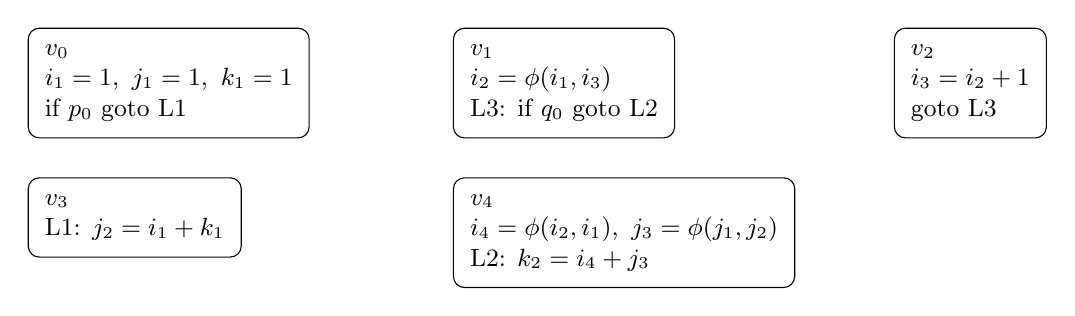
\begin{tikzpicture}[b/.style={draw,rounded corners,align=left,font=\small,inner sep=6pt}]
\node[b,anchor=north west] at (0,0) {$v_0$\\$i_1=1,\ j_1=1,\ k_1=1$\\$\text{if }p_0\text{ goto L1}$};
\node[b,anchor=north west] at (5.4,0) {$v_1$\\$i_2=\phi(i_1,i_3)$\\$\text{L3: if }q_0\text{ goto L2}$};
\node[b,anchor=north west] at (11,0) {$v_2$\\$i_3=i_2+1$\\$\text{goto L3}$};
\node[b,anchor=north west] at (0,-1.9) {$v_3$\\$\text{L1: }j_2=i_1+k_1$};
\node[b,anchor=north west] at (5.4,-1.9) {$v_4$\\$i_4=\phi(i_2,i_1),\ j_3=\phi(j_1,j_2)$\\$\text{L2: }k_2=i_4+j_3$};
\end{tikzpicture}
\end{center}
\end{document}
